\documentclass[11pt,a4paper]{article}
\usepackage[utf8]{inputenc}
\usepackage{amsmath, amssymb}
\usepackage{minted}
\usepackage{booktabs}
\usepackage{tabularx}
\usepackage{tikz}
\usepackage[margin=1in]{geometry}
\usepackage{xcolor}

\newenvironment{important}
    {\vspace{1em}\noindent\begin{tabular}{|p{0.97\textwidth}|}\hline\vspace{0.1em}}
    {\vspace{0.1em}\\\hline\end{tabular}\vspace{1em}}

\newcommand{\sta}{\textbf{\textcolor{red}{[CRITICAL]}} }

\begin{document}
% Lecture Notes: Genome Assembly and Read Mapping Indices
\section{Genome Assembly}

The reconstruction of a genome from short sequencing reads relies heavily on graph-based algorithms. Rather than analyzing overlaps between entire reads—which requires extremely high sequencing depth to capture reads shifted by single bases—reads are decomposed into smaller overlapping substrings called $k$-mers.

\subsection{K-mers and Overlap Requirements}
To merge two biological sequences, they must share a minimum acceptable overlap. If we define $\theta$ as the minimum overlapping fraction of a read's length, the absolute required overlap is $\theta \times \text{length}$. Instead of explicitly computing alignments for every read overlap, we decompose reads into smaller segments. 

\textbf{Example:} K-mer overlapping
Given two reads of length 12, we can decompose them into 6-mers. If the end 6-mer of the first read is identical to the beginning 6-mer of the second read, we know the reads share an overlap of exactly 5 bases (because a $k$-mer transition represents an overlap of $k-1$ bases).
This illustrates the direct relationship between chosen $k$-mer size and the minimum read overlap implicitly required to connect sequencing fragments.

\subsection{De Bruijn Graphs in Assembly}

\begin{important}
\textbf{De Bruijn Graph}: A directed graph representing overlaps between sequences. An original string is decomposed into a collection of $k$-mers, which act as directed edges between nodes. The nodes correspond to the $(k-1)$-mer prefixes and suffixes of those edges.
\end{important}

To construct the graph from a set of reads:
\begin{enumerate}
    \item Decompose each sequence into all possible $k$-mers.
    \item Create a node for every $(k-1)$-mer prefix and suffix.
    \item Draw a directed edge corresponding to the $k$-mer from its prefix node to its suffix node.
    \item Merge all identical nodes, preserving all distinct incoming and outgoing edges.
\end{enumerate}

\begin{center}
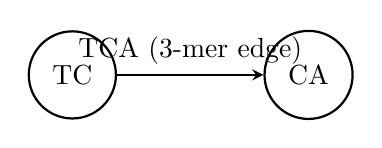
\begin{tikzpicture}[node distance=3cm, >=stealth, thick]
    \node[draw, circle, inner sep=0.2cm] (1) {TC};
    \node[draw, circle, inner sep=0.2cm, right of=1] (2) {CA};
    \draw[->] (1) -- node[above] {TCA (3-mer edge)} (2);
\end{tikzpicture}
\end{center}

By merging identical nodes, the graph compactly represents the topology of the genome. \sta An unambiguous path (a sequence of nodes where each has exactly an in-degree of 1 and an out-degree of 1) can be mathematically compressed by merging the sequential nodes into a single, longer sequence node, greatly simplifying the graph for pathfinding.

\subsection{Eulerian vs. Hamiltonian Paths}
To reconstruct the original string, we must traverse the graph. There are two primary paradigms:
\begin{itemize}
    \item \textbf{Hamiltonian Path}: A path visiting every \textit{node} exactly once. Finding this path is NP-complete, making it computationally infeasible for large genomes.
    \item \textbf{Eulerian Path}: A path visiting every \textit{edge} exactly once. Because we map $k$-mers to edges, visiting every edge precisely rebuilds the original sequences. This can be solved in linear time, which is why modern genome assemblers rely on Eulerian paths over De Bruijn graphs.
\end{itemize}

\begin{important}
\textbf{Property (Eulerian Traversal Rules):} The existence of an Eulerian path or cycle depends strictly on the degrees of the vertices.
\begin{itemize}
    \item \textbf{Undirected Graphs}: 
        \begin{itemize}
            \item \textit{Cycle}: The degrees of all vertices are even.
            \item \textit{Path}: Exactly two vertices have an odd degree.
        \end{itemize}
    \item \textbf{Directed Graphs} (Applicable to De Bruijn Assembly):
        \begin{itemize}
            \item \textit{Cycle}: $\text{In-degree} = \text{Out-degree}$ for all nodes.
            \item \textit{Path}: Exactly one node has $\text{Out-degree} = \text{In-degree} + 1$ (the start node), exactly one node has $\text{In-degree} = \text{Out-degree} + 1$ (the end node), and all other nodes have balanced degrees.
        \end{itemize}
\end{itemize}
\end{important}

\subsection{Hierholzer's Algorithm}
Hierholzer's Algorithm finds an Eulerian path in a directed graph in linear time, $O(|E|)$.

\begin{enumerate}
    \item \textbf{Verify Prerequisites}: Ensure the graph is connected and satisfies the degree requirements for a directed Eulerian path. Identify the start node (the one with the single extra outgoing edge).
    \item \textbf{Initialize Stacks}: Create a Temporary Stack (\texttt{T}) and a Final Path Stack (\texttt{F}).
    \item \textbf{Start Traversal}: Push the start vertex $v$ onto \texttt{T}.
    \item \textbf{Loop}: While \texttt{T} is not empty:
    \begin{enumerate}
        \item Let $u$ be the vertex at the top of \texttt{T} (do not pop it yet).
        \item If $u$ has unvisited outgoing edges:
        \begin{itemize}
            \item Randomly select an unvisited edge $(u, x)$.
            \item Mark $(u, x)$ as visited (or delete it).
            \item Push vertex $x$ onto \texttt{T}.
        \end{itemize}
        \item If $u$ has \textbf{no} unvisited outgoing edges:
        \begin{itemize}
            \item Pop $u$ from \texttt{T} and push it onto \texttt{F}.
        \end{itemize}
    \end{enumerate}
    \item \textbf{Result Generation}: Pop elements sequentially from \texttt{F} to read the exact Eulerian path. The start node will naturally end up at the top of \texttt{F}, and the end node at the bottom.
\end{enumerate}

% [IMAGE: Directed graph showing step-by-step stack resolution in Hierholzer's Algorithm, illustrating backtracking when a node exhausts its outgoing edges.]

\subsection{Practical Assembly Challenges}
While De Bruijn graph traversal is theoretically elegant, real biological data introduces complexities:
\begin{itemize}
    \item \textbf{Choosing $k$}: A short $k$-mer size fails to span repeating regions, causing the graph to tangle. A large $k$-mer size ensures uniqueness but drastically increases memory requirements and demands significantly higher sequence coverage.
    \item \textbf{Sequencing Errors}: A single base error in a read produces $k$ distinct incorrect $k$-mers. These appear as low-frequency edges (tips or bubbles) in the graph and must be structurally pruned based on coverage cutoffs.
    \item \textbf{Repetitive Regions}: Identical $k$-mers from distant genomic loci merge into single heavily trafficked nodes, obscuring the true linear sequence.
    \item \textbf{Ploidy and Strandedness}: Genomes often contain divergent alleles, requiring tools to separate homologous paths. Additionally, sequenced reads could originate from the forward or reverse complement strand, mandating that both a $k$-mer and its reverse complement be merged into the graph representation.
\end{itemize}


\section{Read Mapping Indices}

Mapping millions of short reads to a 3-billion base-pair human genome requires an index much faster than naive alignment. Suffix-based indices enable search times proportional to the length of the \textit{read}, not the genome.

\subsection{Suffix Trees}
A Suffix Try contains every suffix of an original string as a path from the root to a leaf. Because any substring is the prefix of some suffix, searching for a pattern $P$ of length $N$ takes $O(N)$ comparisons starting from the root.

To avoid the exponential space explosion of a Try, unambiguous paths are compressed into single edges to form a \textbf{Suffix Tree}. Edge labels are replaced by two integers representing the original offset and substring length.
\sta A Suffix Tree reduces the node count to $O(M)$ (where $M$ is genome length). However, structural overhead requires 12.5 to 20 bytes per node, making it too large (over 60 GB) to comfortably index the human genome in standard RAM.

% [IMAGE: A Generalized Suffix Tree illustrating the indexing of multiple concatenated strings ("banana$" and "anana#") using unique termination characters.]

\subsection{Suffix Arrays}

\begin{important}
\textbf{Suffix Array (SA)}: An array of integers representing the starting positions (indices) of all suffixes of an input string, sorted in lexicographical order.
\end{important}

Instead of storing massive tree structures, an SA stores only 4 bytes per character. 
Because suffixes are sorted, identical substrings are grouped together in consecutive blocks. A binary search on a Suffix Array takes $O(|P| \log M)$ time to locate read matches.

\textbf{Construction (Prefix Doubling in $O(M \log M)$)}:
Naively sorting suffixes takes $O(M^2 \log M)$. A far more efficient recursive approach is:
\begin{enumerate}
    \item Sort suffixes by their first character (blocks of A, C, G, T).
    \item For phase $i$, double the sorting scope. If suffixes are sorted by their first $2^{i-1}$ characters, their order by $2^i$ characters can be determined in linear time by simply looking up the ranks computed in the previous step.
    \item Terminate when the sorted length exceeds $M$. This requires $O(\log M)$ phases, yielding $O(M \log M)$ complexity.
\end{enumerate}

\subsection{Burrows-Wheeler Transform (BWT)}

\begin{important}
\textbf{Burrows-Wheeler Transform (BWT)}: A reversible string transformation algorithm that rearranges characters into runs of identical letters, facilitating both efficient compression (e.g., bzip2) and rapid indexing.
\end{important}

\textbf{Construction via Rotations (Naive Method)}:
\begin{enumerate}
    \item Append a termination character \texttt{\$} (lexicographically smallest) to the input string $T$.
    \item Generate all $|T|$ cyclic rotations of the string.
    \item Sort the rotations lexicographically to form the BWT Matrix.
    \item The last column of this matrix is the BWT string ($L$).
\end{enumerate}

\begin{table}[h]
\centering
\caption{BWT Matrix Generation for $T = \text{abracadabra\$}$}
\label{tab:bwt}
\begin{tabularx}{0.7\textwidth}{l X}
\toprule
\textbf{F (First Column)} & \textbf{L (Last Column)} \\
\midrule
\texttt{\$} & \texttt{a b r a c a d a b r} \textbf{\texttt{a}} \\
\texttt{a} & \texttt{\$ a b r a c a d a b} \textbf{\texttt{r}} \\
\texttt{a} & \texttt{b r a \$ a b r a c a} \textbf{\texttt{d}} \\
... & ... \\
\bottomrule
\end{tabularx}
\end{table}

\textbf{Direct Relationship Between Suffix Array and BWT}:
Sorting full rotations is computationally identical to sorting suffixes (the termination character uniquely limits comparative depth). Therefore, the position of a rotation in the BWT matrix matches the corresponding suffix position in the Suffix Array. 

We can compute the BWT directly from the SA in linear time $O(M)$ without generating matrices:
\begin{equation}
BWT[i] = 
\begin{cases} 
T[SA[i] - 1] & \text{if } SA[i] \neq 0 \\
\texttt{\$} & \text{if } SA[i] = 0 
\end{cases}
\end{equation}
This formula holds because the character in the last column of a sorted rotation is simply the character immediately preceding the suffix in the original string.

\subsection{The FM Index}
The FM Index uses the BWT string, the Suffix Array, and specific checkpoints to index a genome in a highly memory-efficient manner.

\begin{itemize}
    \item \textbf{Memory Footprint}: The FM index compresses the human genome to approximately 1.5 GB, avoiding the 12+ GB required by a raw suffix array or 60+ GB required by a suffix tree.
    \item \textbf{Checkpointing (Selective Suffix Array)}: Rather than storing all $M$ integers of the Suffix Array, the FM Index stores only every $k^{th}$ value. 
    \item \textbf{LF Mapping}: The index heavily relies on the Last-to-First mapping property of the BWT: the $i^{th}$ occurrence of a character in the last column ($L$) corresponds to the exact same original character as the $i^{th}$ occurrence of that character in the first column ($F$).
    \item \textbf{Retrieval}: To find the original genomic coordinate of a mapped read, we utilize LF mapping to "hop" backward through the genome until we hit a checkpointed $k^{th}$ index in the selective Suffix Array, requiring at most $k-1$ resolution steps.
\end{itemize}

\end{document}